\documentclass{article}

% ==================== بسته‌های کتابخانه ====================

% -- مدیریت مراجع با پشتیبانی از natbib --
\usepackage[backend=biber,style=ieee,sorting=none,natbib]{biblatex}  % <-- گزینه natbib اضافه شد
\addbibresource{RecommendationBib.bib}

% -- ریاضیات --
\usepackage{amsmath}
\usepackage{amssymb}

% -- قضایا، تعاریف، فرضیات و نکات --
\usepackage{amsthm}

\theoremstyle{plain}
\newtheorem{proposition}{Proposition}
\newtheorem{lemma}{Lemma}
\newtheorem{theorem}{Theorem}
\newtheorem{assumption}{Assumption}

\theoremstyle{definition}
\newtheorem{definition}{Definition}
\newtheorem{example}{Example}

\theoremstyle{remark}
\newtheorem{remark}{Remark}

% -- تصاویر و جداول --
\usepackage{graphicx}
\usepackage{multirow}
\usepackage{booktabs}
\usepackage{subcaption}
\usepackage{caption}
\usepackage{float}

% -- تنظیمات صفحه --
\usepackage{geometry}
\geometry{margin=1in}

% -- الگوریتم‌ها --
\usepackage{algorithm}
\usepackage{algorithmic}

% -- رسم شکل با تیک‌زد --
\usepackage{tikz}
\usetikzlibrary{positioning, shapes.geometric, arrows.meta, fit}

% -- تنظیمات استایل تیک‌زد --
\tikzset{
	process/.style={rectangle, draw=blue!60, fill=blue!10, very thick, minimum height=1cm, minimum width=3.5cm, text centered, rounded corners},
	io/.style={rectangle, draw=blue!60, fill=blue!5, very thick, minimum height=1cm, minimum width=4cm, text centered, rounded corners},
	arrow/.style={thick,->,>=Stealth}
}




%opening
\title{Bayesian Clustering with User-Side Information for Streaming Recommender Systems: Addressing Data Sparsity and Cold-Start with Provable Convergence}
\author{}

\begin{document}

\maketitle

\begin{abstract}
Collaborative filtering, a popular technique in recommendation systems, faces primary challenges: data sparsity, cold-start limitations, and an inability to adapt to streaming data in real-world environments. Although existing heuristic and distance-based approaches partially address streaming scenarios, they lack theoretical rigor and fail to leverage evolving user-item interactions effectively. This study introduces a novel Bayesian clustering framework that integrates user-side information with probabilistic priors to overcome these challenges. 
The proposed clustering method reduces the impact of rating matrix sparsity by leveraging prior knowledge for streaming data. Furthermore, incorporating user-side information mitigate the effects of the cold-start problem on prediction accuracy.
The convergence of the proposed clustering method is established in this study through the proof that the Hessian matrix of its objective function is positive definite. Empirical validation demonstrates a faster convergence rate of proposed method compared to the Fuzzy C-Means. The experimental results on real-world streaming datasets (MovieLens, yelp) indicate that the proposed method, in addition to overcoming the limitations, achieves higher accuracy in predicting user ratings than other methods. By integrating Bayesian inference with the ability to adapt to streaming data, this study addresses key limitations in current recommender systems research. 

\textbf{Keywords}:Bayesian Clustering, Streaming Data, Collaborative Filtering, Cold-Start Mitigation, Data Sparsity, Convergence Analysis, Side Information, Recommendation Systems.
\end{abstract}

\section{Introduction}
Every piece of knowledge builds upon another, and the understanding of any truth requires awareness of its foundation. 
Recommender systems, much like the evolution of knowledge, build upon prior information to refine and enhance decision-making. These systems aim to maximize user satisfaction by generating a list of the most relevant and personalized items. Given their significance, extensive research has been conducted in this domain, exploring various methodologies to improve recommendation quality. Each approach relies on different sources of information, benefiting from past interactions to predict future preferences. However, much like gaps in historical knowledge challenge understanding, recommender systems also struggle with incomplete data, cold-start issues, and the dynamic nature of evolving user-item interactions.

Recommender systems aim to enhance user satisfaction by generating a list of the most relevant and personalized items. Given their significance, extensive research has been conducted in this domain, exploring various methodologies for improving recommendation quality. Each approach leverages different types of information and comes with its own advantages and limitations.  

\underline {\textbf{challenge 1:}}
Despite substantial advancements, recommender systems still face critical challenges rooted in the nature of user–item interaction data, including the cold-start problem, data sparsity, and imbalance \cite{li2024recent, rama2019deep}. These limitations reduce prediction accuracy, preventing the system from effectively tailoring recommendations to user preferences.

\underline{\textbf{challenge 2:}}
 Many existing models assume a static dataset, whereas in real-world scenarios, data arrives continuously in a streaming manner. The ability to handle such dynamic data influx remains a pressing challenge, as most traditional approaches lack adaptability to evolving user-item interactions.  

To address these limitations, this paper proposes a Bayesian clustering framework for streaming recommendation that addresses sparsity and cold-start by leveraging user-side information. we derive an update rule with provable convergence guarantees, ensuring that the model adapts stably as the data stream evolves. This model enhances both the accuracy and adaptability of recommender systems.

The remainder of this paper is organized as follows. Section 2 reviews the literature on content-based, collaborative methods, with a detailed focus on clustering-based CF and the use of side information. Section 3 details the proposed method, including the clustering techniques employed and their integration into the recommender system. Section 4 presents the evaluation of the system’s performance, offering a comparative analysis with existing methods. Finally, Section 5 concludes the study and suggesting directions for future research.

\section{Related Work}
Methods in recommender systems are included three main categories content-based methods, collaborative Filtering(CF), and Hybrid methods \cite{aljunid2025collaborative}. Content-based methods generate recommendations solely based on a user's past behavior and interests, without considering other users' interactions. While simple to implement, they provide a limited selection of similar items and fail to leverage relationships between users. 

Collaborative filtering focuses on user-item interactions rather than item characteristics, recommending items based on the preferences of similar users. This approach enables more diverse and personalized recommendations by utilizing shared user behaviors and preferences \cite{isinkaye2023matrix}. Collaborative methods have two types of algorithms, memory-based and model-based.

In memory-based methods, which are also called neighborhood-based methods, the relationship between users and items is investigated. User-based \cite{zhao2010user,valcarce2019collaborative} or item-based \cite{sarwar2001item,fu2018attention} similarity is considered to predict the user's rating of items that he has not seen before. The primary limitation of memory-based methods is their reliance on loading the entire rating matrix into memory for each prediction, making them inefficient for large-scale datasets in terms of time and memory usage. 

Model-based methods address this issue by employing a predictive model  based on past user-item interactions. Various machine learning algorithms can be utilized in model-based approaches to enhance recommendation accuracy and efficiency. These mainly includes approaches like Matrix factorization \cite{isinkaye2023matrix,shi2020user,yang2018enhancing, behera2023mixed}, Bayes classifier \cite{valdiviezo2019collaborative}, neural networks \cite{wang2015collaborative,angel2022deep,li2017collaborative}.
This paper focuses on common challenges in recommender systems and clustering algorithms. Clustering techniques are commonly used to mitigate the sparsity problem and improve the scalability of CF methods. By grouping users or items with similar characteristics, clustering-based CF systems enhance recommendation performance while reducing computational complexity. 
\begin{itemize}
\item[a) ] Clustering-based Collaborative Filtering \\
Clustering algorithms such as k-means\cite{dakhel2011new, zahra2015novel, ranjan2018category, kant2017leaderrank} and FCM\cite{birtolo2013advances} are widely utilized in recommender systems. Studies have explored various user clustering approaches, including Bayesian matrix factorization \cite{bobadilla2018recommender}, evolutionary clustering that adapts user states over time \cite{liji2018improved}, and weighted clustering that assigns higher importance to users with more interactions \cite{salah2015dynamic}. In \cite{katarya2018recommender}, a hybrid method used gray wolf optimization for initializing clusters, followed by fuzzy c-means (FCM) for user classification based on rating similarity .
Similarly, for item clustering, in \cite{deng2019novel}, an improved Kullback-Leibler divergence is employed to measure item similarity based on probability distributions. In \cite{kant2017leaderrank}, the k-means algorithm is utilized to cluster items, and an item's score is predicted solely based on the average scores of other items within the same cluster. Several methods have been proposed for clustering both users and items. Other approaches include power fuzzy clustering using an exponential fitness function to refine membership \cite{treerattanapitak2012exponential} and network-based clustering where evolving statuses lead to stable groups \cite{chen2017evolutionary}. Clustering via the QUBIC (A Qualitative Biclustering algorithm) in \cite{singh2018impact}, aim to group similar users and items effectively. \cite{science2018dynamic} constructs a network that integrates user characteristics, item features, and temporal information, subsequently applying a dynamic evolutionary clustering algorithm.

Several advanced clustering-aware approaches such as \cite{rajput2025nsga}, proposes an NSGA-II-optimized deep autoencoder framework improve multi-criteria recommendations by optimizing model parameters through a multi-objective approach, addressing data sparsity and non-linearity. \cite{li2025self} presents a self-supervised graph Transformer (SGTN) that improves user-item representations by encoding ratings and applying contrastive learning. It focuses on capturing social and collaborative relationships through decentralized graphs and edge-aware attention. Although not explicitly designed for clustering, it enhances user embeddings, enabling dynamic and context-sensitive user-item grouping in recommendation systems. In \cite{qian2025ifm} a framework that uses adversarial features from multiple models is proposed to improve transferability and enhance user-item representations. It refines embeddings by reducing noise and improving cluster separability, offering a strategy for robust clustering in dynamic recommendation systems. \cite{he2025fedai} presents FedAI, a federated recommendation system that combines spectral clustering and K-means to group users while ensuring privacy. High-order interactions enhance embeddings, improving clustering in decentralized settings without accessing raw data.


\item[b) ] Clustering based on User-side Information \\ 
While clustering-based methods address scalability and sparsity issues in the score matrix, the high dimensionality of user-item data makes them computationally expensive. To mitigate this, many approaches leverage side information as clustering features, significantly reducing the feature space and improving efficiency. \cite{liji2018improved} employs user attributes such as age, gender, and residence to calculate feature distances for clustering. Similarly, \cite{chen2019n2vscdnnr} forms a bipartite user-item graph and converts each node into a vector before clustering. Additionally, \cite{zhao2017coarse} clusters users based on social network labels and items via a bipartite graph, \cite{sheugh2018novel} creates a two-dimensional similarity graph of users for clustering, and \cite{wasid2018clustering} incorporates social information alongside the score matrix to enhance user clustering. Gong et al. \cite{gong2010collaborative} leveraged both explicit ratings and implicit user behavior to improve similarity measurements. Lu et al. \cite{lu2021novel} addressed the sparsity problem in user-item interactions by grouping items with similar features, thereby aligning recommendations more closely with user interests. Additionally, Wasid et al. \cite{wasid2018improved} refined traditional collaborative filtering through a multi-criteria clustering approach, which integrates various aspects of user preferences to yield more diverse and accurate recommendations. Additionally, Mahalanobis distance is employed to measure the similarity between users' score vectors, taking into account not only the given scores but also their variance and covariance \cite{deng2019neural} used variational autoencoders and side information to mitigate data sparsity and the cold start problem. 

\item[c) ] Recommendation in Streaming Data Environment \\
Furthermore, most of clustering-based methods often do not consider streaming data, making them less effective in dynamic environments. With the increasing need for real-time recommendations, online recommender systems have become essential for handling streaming data. These systems must efficiently update user preferences and item interactions as new information becomes available. Recommender systems in e-commerce and digital service platforms must continuously process new users and items, making real-time data handling essential. However, most existing systems rely on fixed datasets for evaluation, limiting their applicability in dynamic environments. Traditional content-based and memory-based collaborative filtering methods require loading all data into memory, making them unsuitable for streaming data. In contrast, model-based collaborative filtering, particularly matrix decomposition methods like ALS and SGD, allows incremental updates. While these methods address some streaming challenges, they remain computationally expensive and risk losing information during model updates. Clustering-based recommender systems for streaming data mainly rely on heuristics without leveraging prior knowledge, limiting their effectiveness. For instance, distance-based clustering adjusts noisy data positioning \cite{georgieva2008dynamic}, as well as a density-based method updates clusters dynamically using local averages\cite{baruah2012evolving}. In \cite{das2007google} an online model proposed for Google News, continuously updates recommendations based on user interactions, ensuring that personalized news suggestions remain relevant. A streaming matrix‐factorization framework proposed in \cite{jakomin2020simultaneous} that incrementally fuses multiple heterogeneous data streams to continuously adapt latent user‐item representations and mitigate both data sparsity and cold‐start issues. While online recommender systems rely on user feedback, new users, and new items for updates, many clustering-based methods struggle with streaming data. Integrating online learning into clustering-based collaborative filtering can improve adaptability in dynamic environments.
\end{itemize}

One of the primary strategies for mitigating data sparsity is cluster-based collaborative filtering. Clustering-based recommender systems can enhance recommendation reliability while maintaining lower computational complexity. Despite the benefits of clustering-based CF methods, challenges remain. Feature selection for clustering is a critical issue, as high-dimensional user-item matrices can lead to the curse of dimensionality. Conversely, clustering based on side features alone may not accurately capture user interests, reducing prediction accuracy. In addition, deal with streaming data, making them effective in dynamic environments is rally important.

To address these limitations, a Bayesian clustering model is introduced, incorporating prior knowledge for streaming data clustering. Unlike traditional clustering approaches, this method dynamically updates user and item clusters as new interactions occur. By combining user ratings with side features, the model improves personalization, incorporates real-time updates to handle user feedback, new users, and alleviates the cold start problem by leveraging additional user information beyond the rating matrix. Experimental results demonstrate that this approach outperforms existing clustering-based CF models in terms of accuracy and efficiency, making it well-suited for real-time recommendation systems. 
















%------------------------------







%------------------------------
\section{Proposed Method}
\label{sec:proposed_method}

\subsection{Overview: A Latent Recommendation Perspective}
\label{subsec:overview}

The proposed recommender is organized around a single unifying idea: instead of mapping a user or item directly onto a recommendation set, the model routes this mapping through an intermediate space of \emph{latent taste prototypes}. This is conceptually related to neighborhood-based and matrix-factorization collaborative filtering, where user/item affinities are explained through a small number of latent factors, and to mixture-of-experts style recommenders, where each ``expert'' (here, a hidden component $c_i$) specializes in a sub-population of user behavior. The key departure from classical latent-factor CF is that our latent layer is explicitly \emph{probabilistic and two-stage}: (i) a Bayesian filtering stage infers how strongly an incoming item/user activates each latent prototype, and (ii) a Bayesian decoding stage infers how strongly each activated prototype supports a given candidate set. The final relevance score is obtained by marginalizing over all latent prototypes, which yields a soft, uncertainty-aware generalization of hard cluster assignment. Section~\ref{subsec:latent_filtering} develops this general formulation and Section~\ref{subsec:theory_general} establishes its formal statistical properties; Sections~\ref{subsec:bridge}--\ref{subsec:rating_prediction} instantiate it into a concrete streaming user-clustering and rating-prediction pipeline; Section~\ref{subsec:theory} establishes convergence guarantees for the resulting streaming optimization procedure.

\subsection{Latent Filtering Formulation}
\label{subsec:latent_filtering}

Let $x \in \mathcal{X}$ denote an incoming item (or user) for which the system must identify the most relevant candidate set among
\[
\mathcal{S}_1, \mathcal{S}_2, \ldots, \mathcal{S}_K, \qquad \mathcal{S}_j \subseteq \mathcal{X},
\]
where each $\mathcal{S}_j$ represents a set of items (or users) sharing a latent recommendation relation. The goal is not merely to assign $x$ to a precomputed cluster, but to infer the relevance of $x$ to each candidate set $\mathcal{S}_j$ under uncertainty and incomplete observation. Each set $\mathcal{S}_j$ is represented by a latent descriptor $\theta_j = (\mu_j, \Sigma_j)$, describing the center and dispersion of the latent representations of items belonging to $\mathcal{S}_j$.

Rather than mapping $x$ directly to $\mathcal{S}_j$, we introduce an intermediate \emph{latent filtering} layer. The incoming item is first encoded into a latent vector
\[
\mathbf{z}(x) = \phi(x) \in \mathbb{R}^d.
\]

\begin{remark}[On the choice of $\phi$]
	\label{rem:phi_choice}
	The parametrization of $\phi$ is deliberately left unspecified at this stage: any mapping $\phi:\mathcal X\to\mathbb R^d$ is admissible in principle, including linear or PCA-type projections, autoencoders, or task-specific deep encoders trained jointly with the prototypes $\{\mathbf m_i\}$. The two-stage decomposition developed below — and its statistical properties in Section~\ref{subsec:theory_general} — hold for any fixed, measurable $\phi$; the concrete choice and end-to-end learning procedure for $\phi$ is deliberately kept outside the scope of the present formulation and is addressed in a companion study.
\end{remark}

The model then estimates the posterior involvement of $x$ in each of $C$ hidden components $c_i$, $i = 1, \ldots, C$:
\[
q_i(x) \triangleq P(c_i \mid x) = P(c_i \mid \mathbf{z}(x)).
\]
This posterior plays the role of a Bayesian filter over the latent space. Each hidden component $c_i$ is represented by a latent prototype and covariance $\psi_i = (\mathbf{m}_i, \Lambda_i)$, with likelihood
\[
p(\mathbf{z}(x) \mid c_i) = \mathcal{N}\big(\mathbf{z}(x); \mathbf{m}_i, \Lambda_i\big).
\]
By Bayes' rule,
\begin{equation}
	\label{eq:posterior_component}
	q_i(x) = P(c_i \mid x) = \frac{\rho_i \, \mathcal{N}(\mathbf{z}(x); \mathbf{m}_i, \Lambda_i)}{\sum_{\ell=1}^{C} \rho_\ell \, \mathcal{N}(\mathbf{z}(x); \mathbf{m}_\ell, \Lambda_\ell)},
\end{equation}
where $\rho_i = P(c_i)$ is the prior probability of the $i$-th hidden component.

After filtering, the relevance of hidden component $c_i$ to candidate set $\mathcal{S}_j$ is evaluated by assessing prototype $\mathbf{m}_i$ under the distribution associated with $\mathcal{S}_j$:
\begin{equation}
	\label{eq:likelihood_prototype}
	f(\mathbf{m}_i \mid \theta_j) = \mathcal{N}(\mathbf{m}_i; \mu_j, \Sigma_j) = \frac{1}{(2\pi)^{d/2} |\Sigma_j|^{1/2}} \exp\!\left( -\frac{1}{2} (\mathbf{m}_i - \mu_j)^T \Sigma_j^{-1} (\mathbf{m}_i - \mu_j) \right).
\end{equation}
Using Bayes' rule, the posterior association between set descriptor $\theta_j$ and hidden component $c_i$ (equivalently, its prototype $\mathbf{m}_i$) is
\begin{equation}
	\label{eq:posterior_set}
	f(\theta_j \mid c_i) \equiv f(\theta_j \mid \mathbf{m}_i) = \frac{f(\mathbf{m}_i \mid \theta_j) \, P(\theta_j)}{\sum_{r=1}^{K} f(\mathbf{m}_i \mid \theta_r) \, P(\theta_r)}.
\end{equation}
The complete inference chain is therefore
\[
x \;\longrightarrow\; \mathbf{z}(x) = \phi(x) \;\longrightarrow\; P(c_i \mid x) \;\longrightarrow\; f(\theta_j \mid c_i) \;\longrightarrow\; \mathcal{S}_j.
\]
The relevance score of $x$ to candidate set $\mathcal{S}_j$ is obtained by marginalizing over all hidden components:
\begin{equation}
	\label{eq:relevance_score}
	R_j(x) = \sum_{i=1}^{C} P(c_i \mid x) \, f(\theta_j \mid c_i),
\end{equation}
and the estimated recommendation set is
\begin{equation}
	\label{eq:estimated_set}
	\widehat{\mathcal{S}}(x) = \mathcal{S}_{\widehat{j}}, \qquad \widehat{j} = \arg\max_{j} \, R_j(x).
\end{equation}
This formulation cleanly separates the two probabilistic roles of the latent space: $P(c_i \mid x)$ measures how strongly the incoming item activates each hidden component, while $f(\theta_j \mid c_i)$ measures how strongly each hidden component supports a given candidate recommendation set. From a recommender-systems standpoint, $P(c_i \mid x)$ plays a role analogous to a soft, learned gating function over latent taste prototypes (as in mixture-of-experts recommenders), while $f(\theta_j \mid c_i)$ plays the role of a probabilistic neighborhood/decoder that converts prototype activations into set-level evidence — generalizing hard nearest-centroid assignment into a fully marginalized, uncertainty-aware score.

\paragraph{Why a latent layer at all.} Directly estimating $P(\mathcal{S}_j \mid x)$ over $K$ candidate sets from a high-dimensional, heterogeneous raw representation $x$ — which may mix ratings, side information, and item content of different types — would in the worst case require a separate estimator per set, with statistical and computational cost growing with $K$. Routing $x$ through a shared latent space $\mathbf{z}(x) = \phi(x)$, followed by a small number $C \ll K$ of latent prototypes, factorizes this estimation problem: the encoder $\phi$ absorbs the heterogeneity and dimensionality of the raw input, while the $C$ prototypes $\{\mathbf{m}_i\}$ capture reusable, coarse-grained modes of variation shared \emph{across all} $K$ candidate sets. Because the prototypes are shared, estimating them costs $O(C)$ statistical parameters rather than $O(K)$, and a newly introduced candidate set $\mathcal{S}_{K+1}$ can be scored via $f(\theta_{K+1} \mid c_i)$ without re-estimating $\phi$ or $\{\mathbf{m}_i\}$. The latent layer is therefore what makes the two-stage decomposition of Eq.~\eqref{eq:relevance_score} statistically economical and inductively transferable to new candidate sets, rather than a merely architectural convenience — a property made precise in Proposition~\ref{prop:sample_efficiency} below.

\begin{figure}[t]
	\centering
	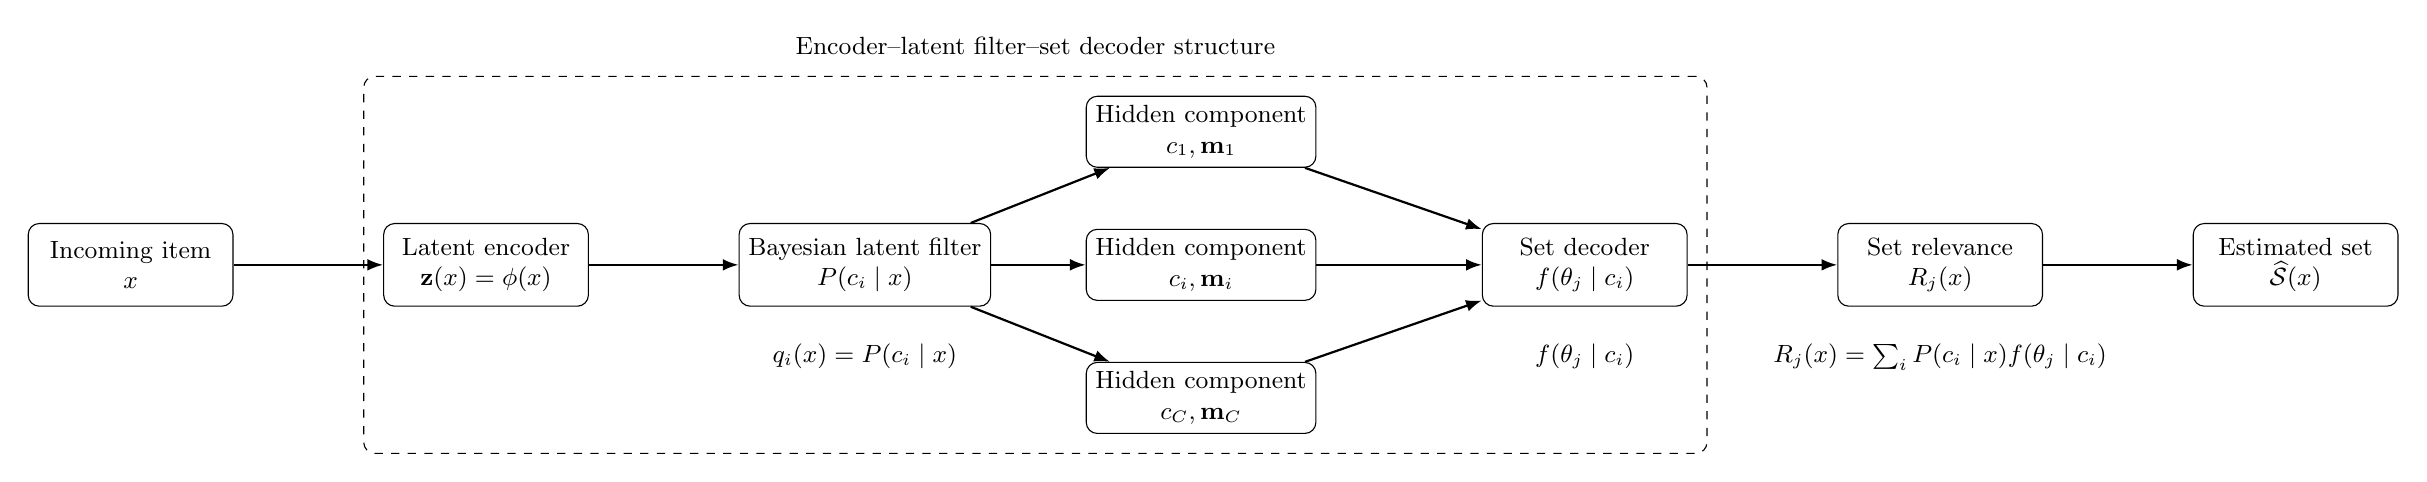
\begin{tikzpicture}[
		node distance=1.55cm and 1.9cm,
		box/.style={draw, rounded corners, align=center, minimum width=2.6cm, minimum height=1.05cm, font=\small},
		smallbox/.style={draw, rounded corners, align=center, minimum width=2.25cm, minimum height=0.9cm, font=\small},
		arrow/.style={-{Latex[length=2mm]}, thick},
		dashedbox/.style={draw, dashed, rounded corners, inner sep=7pt}
		]
		\node[box] (x) {Incoming item\\ $x$};
		\node[box, right=of x] (enc) {Latent encoder\\ $\mathbf{z}(x)=\phi(x)$};
		\node[box, right=of enc] (filter) {Bayesian latent filter\\ $P(c_i\mid x)$};
		
		\node[smallbox, above right=0.7cm and 1.2cm of filter] (c1) {Hidden component\\ $c_1,\mathbf{m}_1$};
		\node[smallbox, right=1.2cm of filter] (ci) {Hidden component\\ $c_i,\mathbf{m}_i$};
		\node[smallbox, below right=0.7cm and 1.2cm of filter] (cC) {Hidden component\\ $c_C,\mathbf{m}_C$};
		
		\node[box, right=2.1cm of ci] (decoder) {Set decoder\\ $f(\theta_j\mid c_i)$};
		\node[box, right=of decoder] (score) {Set relevance\\ $R_j(x)$};
		\node[box, right=of score] (set) {Estimated set\\ $\widehat{\mathcal{S}}(x)$};
		
		\draw[arrow] (x) -- (enc);
		\draw[arrow] (enc) -- (filter);
		\draw[arrow] (filter) -- (c1);
		\draw[arrow] (filter) -- (ci);
		\draw[arrow] (filter) -- (cC);
		\draw[arrow] (c1) -- (decoder);
		\draw[arrow] (ci) -- (decoder);
		\draw[arrow] (cC) -- (decoder);
		\draw[arrow] (decoder) -- (score);
		\draw[arrow] (score) -- (set);
		
		\node[dashedbox, fit=(enc)(filter)(c1)(ci)(cC)(decoder)] (latentbox) {};
		\node[font=\small, above=0.15cm of latentbox] {Encoder--latent filter--set decoder structure};
		
		\node[font=\small, below=0.35cm of filter] (eq1) {$q_i(x)=P(c_i\mid x)$};
		\node[font=\small, below=0.35cm of decoder] (eq2) {$f(\theta_j\mid c_i)$};
		\node[font=\small, below=0.35cm of score] (eq3) {$R_j(x)=\sum_i P(c_i\mid x)f(\theta_j\mid c_i)$};
	\end{tikzpicture}
	\caption{Bayesian latent filtering view of the proposed recommender. The structure is encoder-like because $x$ is first mapped to a latent representation and then filtered through hidden components. It is \emph{not} a classical autoencoder, since the objective is not reconstruction of $x$, but inference of the most relevant recommendation set $\widehat{\mathcal{S}}(x)$.}
	\label{fig:bayesian_latent_filtering}
\end{figure}

\subsection{Statistical Justification of the Latent Marginalization}
\label{subsec:theory_general}

We now formalize the intuition of Section~\ref{subsec:latent_filtering}: introducing the hidden component $c$ is not a heuristic architectural choice, but provably (i) preserves Bayes-optimality of the resulting decision rule under the natural 0--1 loss, and (ii) turns the estimation of $\{\theta_j\}$ into a well-posed maximum a posteriori (MAP) / maximum likelihood (ML) problem, of which the streaming objective of Section~\ref{subsec:user_clustering} is a tractable relaxation.

\begin{assumption}[Sufficiency of the hidden component]
	\label{ass:sufficiency}
	The hidden component $c$ renders $x$ and $\mathcal{S}_j$ conditionally independent, i.e.\ $x \perp \mathcal{S}_j \mid c$: all information carried by $x$ that is relevant to predicting $\mathcal{S}_j$ passes through the posterior $P(c \mid x)$.
\end{assumption}

\begin{proposition}[Bayes-risk optimality of the marginalized relevance rule]
	\label{prop:bayes_optimal}
	Under Assumption~\ref{ass:sufficiency}, the marginalized relevance score of Eq.~\eqref{eq:relevance_score} coincides with the true class posterior, $R_j(x) = P(\mathcal{S}_j \mid x)$ for every $j$. Consequently, for the 0--1 loss risk
	\[
	\mathrm{Risk}(g) = \Pr_{x}\big[g(x) \neq j^\star(x)\big], \qquad j^\star(x) = \arg\max_j P(\mathcal S_j \mid x),
	\]
	the decision rule of Eq.~\eqref{eq:estimated_set}, $\widehat{j}(x) = \arg\max_j R_j(x)$, minimizes $\mathrm{Risk}(g)$ over all measurable decision rules $g:\mathcal X \to \{1,\dots,K\}$; that is, it is the Bayes-optimal (MAP) classification rule for the recommendation task.
\end{proposition}

\begin{proof}
	By the law of total probability and Assumption~\ref{ass:sufficiency},
	\[
	P(\mathcal{S}_j \mid x) = \sum_{i=1}^{C} P(\mathcal{S}_j \mid c_i, x)\,P(c_i \mid x) = \sum_{i=1}^{C} P(\mathcal{S}_j \mid c_i)\,P(c_i \mid x) = \sum_{i=1}^{C} f(\theta_j \mid c_i)\,P(c_i \mid x) = R_j(x),
	\]
	where the middle equality uses conditional independence to drop $x$ from $P(\mathcal S_j\mid c_i,x)$, and the identification $P(\mathcal S_j\mid c_i)\equiv f(\theta_j\mid c_i)$ follows from the definition of the set decoder in Eq.~\eqref{eq:posterior_set}. The optimality of $g^\star(x)=\arg\max_j P(\mathcal S_j\mid x)$ under 0--1 loss is the classical Bayes-classifier theorem \citep[Ch.~2]{devroye1996probabilistic}. Since $R_j(x)=P(\mathcal S_j\mid x)$, the rule of Eq.~\eqref{eq:estimated_set} coincides with $g^\star$ and therefore minimizes $\mathrm{Risk}(g)$.
\end{proof}

Proposition~\ref{prop:bayes_optimal} shows that as long as the hidden component is a sufficient statistic for the recommendation task (Assumption~\ref{ass:sufficiency}), routing inference through $c$ costs nothing in terms of decision-theoretic optimality: the two-stage architecture cannot do worse, in the population limit, than directly modeling $P(\mathcal S_j\mid x)$. Combined with the sample-efficiency argument above, this identifies the precise sense in which adding the latent variable improves the estimation problem.

\begin{proposition}[Statistical economy of the shared latent layer]
	\label{prop:sample_efficiency}
	Let $\mathcal{H}_K$ be the hypothesis class of posteriors $P(\mathcal S_j\mid x)$ modeled directly and independently for each of the $K$ candidate sets, with $p$ free parameters per set, so $\dim(\mathcal H_K)=O(Kp)$. Let $\mathcal{H}_C$ be the hypothesis class induced by Eq.~\eqref{eq:relevance_score} under Assumption~\ref{ass:sufficiency}, with $C\ll K$ shared components $\{\psi_i\}$ ($p$ parameters each) and $K$ light-weight decoders $\{\theta_j\}$ ($p'\ll p$ parameters each), so $\dim(\mathcal H_C) = O(Cp + Kp')$. If $C p + K p' = o(Kp)$ as $K\to\infty$ (e.g.\ $C$ fixed and $p'=O(1)$), then $\dim(\mathcal H_C) = o(\dim(\mathcal H_K))$, and standard uniform-convergence bounds (e.g.\ Rademacher complexity or VC-type bounds) give a strictly smaller generalization gap for the latent-filtered estimator at equal sample size $N$, and, symmetrically, a smaller sample size suffices to reach a target generalization gap.
\end{proposition}

The proof is a direct application of standard capacity-based generalization bounds (e.g.\ \citealt{bartlett2002rademacher}) to the two hypothesis classes and is omitted; the substantive content is the parameter-count comparison $O(Kp)$ vs.\ $O(Cp+Kp')$, which is what the sharing of $\{\psi_i\}$ across all $K$ sets buys in Eq.~\eqref{eq:relevance_score}.

\begin{proposition}[MAP/ML characterization of the training objective]
	\label{prop:map_ml}
	Consider the generative model $\theta_j \sim f(\theta_j)$ and, given assignment to set $j$, $z_i \mid \theta_j \sim \mathcal N(\mu_j,\Sigma_j)$ (Eq.~\eqref{eq:f_likelihood}). For a hard partition $u_{ij}\in\{0,1\}$, $\sum_j u_{ij}=1$, the joint log-posterior of $(\{\theta_j\},\{u_{ij}\})$ given data $\{z_i\}_{i=1}^N$ is, up to an additive constant,
	\[
	\log P(\theta,u\mid z) \;\propto\; \sum_{i=1}^N\sum_{j=1}^C u_{ij}\Big[\log f(z_i\mid \theta_j) + \log f(\theta_j)\Big].
	\]
	As $m\to 1^+$ in the fuzzy objective $J_m$ of Eq.~\eqref{eq:obj_function}, the optimal membership $u_{ij}$ collapses to the hard indicator $\mathbb{1}\{j=\arg\max_k f_{ik}\}$, and $J_1$ coincides exactly with $\exp\big(\log P(\theta,u\mid z)\big)$ above; hence, in this limit, alternating maximization of $J_m$ computes exactly the joint MAP estimate of $(\{\theta_j\},\{u_{ij}\})$ (or the ML estimate, if $f(\theta_j)$ is taken to be flat). For $m>1$, $J_m$ is a maximum-entropy-regularized relaxation of the same objective, replacing the hard indicator with a soft, temperature-controlled responsibility, trading exact MAP optimality for reduced sensitivity to local optima and smoother optimization landscape — the usual bias–variance trade-off of fuzzy/soft variants of hard-assignment EM-type estimators.
\end{proposition}

Together, Propositions~\ref{prop:bayes_optimal}--\ref{prop:map_ml} give the missing formal grounding for the latent construction: Proposition~\ref{prop:bayes_optimal} shows that marginalizing over the hidden component preserves Bayes-optimality of the induced decision rule; Proposition~\ref{prop:sample_efficiency} shows that sharing the hidden component across candidate sets reduces the effective hypothesis-class complexity; and Proposition~\ref{prop:map_ml} identifies the concrete estimator implemented in Section~\ref{subsec:user_clustering} as a (fuzzy relaxation of a) MAP/ML estimator under the assumed hierarchical Gaussian model.

\subsection{From General Relevance Scoring to a Tractable Streaming Instantiation}
\label{subsec:bridge}

The formulation of Section~\ref{subsec:latent_filtering} assumes the hidden-component parameters $\psi_i = (\mathbf{m}_i, \Lambda_i)$ and the set descriptors $\theta_j = (\mu_j, \Sigma_j)$ are already available, so that $P(c_i \mid x)$ and $f(\theta_j \mid c_i)$ can be evaluated directly via Eqs.~\eqref{eq:posterior_component} and~\eqref{eq:posterior_set}. In a real recommender, however, neither is given in advance: both the latent prototypes and the candidate-set descriptors must be estimated from streaming user/item data.

We therefore instantiate the general framework in the regime where hidden components and candidate sets coincide, $C = K$ and $c_j \equiv \mathcal{S}_j$, so that the two-stage relevance score of Eq.~\eqref{eq:relevance_score} collapses to a single learned filter,
\begin{equation}
	\label{eq:collapsed_relevance}
	R_j(x) = f(\theta_j \mid \mathbf{z}(x)),
\end{equation}
and the estimated-set rule of Eq.~\eqref{eq:estimated_set} is unchanged, $\widehat{\mathcal{S}}(x) = \mathcal{S}_{\widehat{j}}$ with $\widehat{j} = \arg\max_j R_j(x)$. Because $\theta_j$ is now unknown, the posterior $P(c_j \mid x)$ cannot be evaluated in closed form as in Eq.~\eqref{eq:posterior_component}; instead, it is \emph{jointly estimated} together with $\theta_j$ through a relaxed, fuzzy surrogate $u_{ij} \in [0,1]$ that plays the same role as $P(c_j\mid x_i)$ but is optimized rather than computed — this is precisely the $m>1$ relaxation of the MAP objective identified in Proposition~\ref{prop:map_ml}. This yields the training objective
\[
\max_{u,\,\theta} \; \sum_{j=1}^{K} \sum_{i=1}^{N} u_{ij}^{m} \, R_j(x_i), \qquad 1 < m < \infty,
\]
which is exactly the quantity developed below, first for fixed items (Section~\ref{subsec:item_clustering}) and then for streaming users, where the candidate-set descriptors $\theta_j$ are updated online as new evidence arrives (Section~\ref{subsec:user_clustering}). Sections~\ref{subsec:distributed_clustering}--\ref{subsec:rating_prediction} extend this instantiation with graph-based smoothing of the estimated $\theta_j$ and a rating-prediction rule built directly on $R_j(x)$; Section~\ref{subsec:theory} then establishes convergence guarantees for the resulting alternating estimator.

\subsection{A Concrete Instantiation of the Item-Side Filter}
\label{subsec:item_clustering}

Any estimator of the hidden-component posterior in Eq.~\eqref{eq:posterior_component} is compatible with the general framework, provided it returns a valid probability vector over $C$ components. As a simple, fully unsupervised instantiation for the fixed item-side population, we realize $P(c_i \mid x)$ through the classical Fuzzy C-Means (FCM) membership rule, which recovers $C$ item-side prototypes $\{\mathbf{m}_i\}$ by minimizing
\begin{equation}
	J = \sum_{k=1}^{C} \sum_{i=1}^{n} u_{ki}^m \| x_i - \mu_k \|^2, \qquad u_{ki} \in [0,1],\ m>1.
\end{equation}
This closed-form, low-overhead choice is only one admissible instantiation among several (a Gaussian mixture model or a learned soft-assignment network would serve equally well); replacing it with any other consistent estimator of $P(c_i \mid x)$ leaves the marginalization of Eq.~\eqref{eq:relevance_score} — and the guarantees of Section~\ref{subsec:theory_general} — unaffected. The resulting item-side prototypes serve as fixed reference points for the streaming user-side instantiation developed next.

\subsection{Streaming Bayesian Realization of the Set Descriptors}
\label{subsec:user_clustering}

Users, unlike items, arrive continuously, so the set descriptors $\theta_j$ of Eq.~\eqref{eq:collapsed_relevance} cannot be estimated once and fixed; they must be realized online. Rather than retaining all historical data, the proposed method maintains, for each candidate set $j$, only its current descriptor $\theta_j = (\mu_j, \Sigma_j)$, updated incrementally as new users are observed — an online, memory-efficient realization of $R_j(x)$.

\subsubsection{Objective Function}

Let $z_i = \phi(x_i) \in \mathbb{R}^d$ denote the latent feature vector of user $i$ (Section~\ref{subsec:latent_filtering}), formed by concatenating their rating vector and side-feature vector,
\[
\mu_j = \big\langle [\,r_{\mu j1}, r_{\mu j2}, \ldots, r_{\mu jC}\,;\; f_{\mu j1}, \ldots, f_{\mu jK}\,] \big\rangle .
\]
Substituting the collapsed relevance score $R_j(x_i) = f(\theta_j \mid z_i)$ into the training objective of Section~\ref{subsec:bridge} gives
\begin{equation}
	\label{eq:first}
	\max_{u,\theta_j} \sum_{j=1}^{C} \sum_{i=1}^{N} u_{ij}^m \, f(\theta_j \mid z_i), \qquad 1 < m < \infty.
\end{equation}
By Bayes' theorem, Eq.~\eqref{eq:first} is rewritten as
\begin{equation}
	\label{eq:bayes}
	\max_{u,\theta_j} \sum_{j=1}^{C} \sum_{i=1}^{N} u_{ij}^m \, f(z_i \mid \theta_j) \, f(\theta_j), \qquad 1 < m < \infty,
\end{equation}
where $f(z_i \mid \theta_j)$ is the likelihood of user $i$'s latent vector under set $j$'s descriptor, and $f(\theta_j)$ is the prior over that descriptor — as formalized in Proposition~\ref{prop:map_ml}, Eq.~\eqref{eq:bayes} is precisely the joint MAP/ML objective under a fuzzy ($m>1$) relaxation. Assuming both terms are Gaussian,
\begin{align}
	f(z_i \mid \theta_j) &\sim \mathcal{N}(z_i; \mu_j, \Sigma_j) = \frac{1}{(2\pi)^{d/2} |\Sigma_j|^{1/2}} \exp\!\left( -\frac{1}{2} (z_i - \mu_j)^T \Sigma_j^{-1} (z_i - \mu_j) \right), \label{eq:f_likelihood} \\
	f(\theta_j) &\sim \mathcal{N}(\mu_j; \mu_{\theta_j}, \Sigma_{\theta_j}) = \frac{1}{(2\pi)^{d/2} |\Sigma_{\theta_j}|^{1/2}} \exp\!\left( -\frac{1}{2} (\mu_j - \mu_{\theta_j})^T \Sigma_{\theta_j}^{-1} (\mu_j - \mu_{\theta_j}) \right), \label{eq:f_theta_prior}
\end{align}
where $\mu_{\theta_j}$ and $\Sigma_{\theta_j}$ are the mean and covariance of the prior over $\theta_j$, carried over from the previous streaming step. Substituting Eqs.~\eqref{eq:f_likelihood}--\eqref{eq:f_theta_prior} into~\eqref{eq:bayes} gives the streaming objective
\begin{equation}
	\label{eq:obj_function}
	\begin{split}
		J_m(u_{11}, \ldots, u_{NC}, \theta_1, \ldots, \theta_C) = \sum_{j=1}^{C} \sum_{i=1}^{N} \frac{u_{ij}^m}{2\pi \, |\Sigma_j|^{1/2} |\Sigma_{\theta_j}|^{1/2}} \\
		\times \exp\!\left( -\frac{1}{2} \Big( (z_i - \mu_j)^T \Sigma_j^{-1} (z_i - \mu_j) + (\mu_j - \mu_{\theta_j})^T \Sigma_{\theta_j}^{-1} (\mu_j - \mu_{\theta_j}) \Big) \right).
	\end{split}
\end{equation}

\subsubsection{Update Equations}

Incorporating the constraint $-\sum_{i=1}^{N} \lambda_i \big(\sum_{j=1}^{C} u_{ij} - 1\big)$ via a Lagrangian and differentiating with respect to each parameter yields the update rules below. For clarity, define the auxiliary quantities
\begin{align}
	f_{ij} &= \exp\!\left( -\frac{1}{2} \Big( (z_i - \mu_j)^T \Sigma_j^{-1} (z_i - \mu_j) + (\mu_j - \mu_{\theta_j})^T \Sigma_{\theta_j}^{-1} (\mu_j - \mu_{\theta_j}) \Big) \right), \label{eq:aux_f} \\
	S &= \frac{\Sigma_j^{-1}}{\Sigma_j^{-1} + \Sigma_{\theta_j}^{-1}}, \qquad 1 - S = \frac{\Sigma_{\theta_j}^{-1}}{\Sigma_j^{-1} + \Sigma_{\theta_j}^{-1}}. \label{eq:aux_S}
\end{align}
The set descriptor's mean is updated as a Bayesian-weighted combination of the evidence-driven estimate and the prior,
\begin{equation}
	\label{eq:update_mean}
	\mu_j = S \cdot \frac{\sum_{i=1}^{N} u_{ij}^m f_{ij} z_i}{\sum_{i=1}^{N} u_{ij}^m f_{ij}} \;+\; (1 - S) \cdot \mu_{\theta_j},
\end{equation}
the covariance as
\begin{equation}
	\label{eq:update_cov}
	\Sigma_j = \frac{\sum_{i=1}^{N} u_{ij}^m (z_i - \mu_j)(z_i - \mu_j)^T f_{ij}}{\sum_{i=1}^{N} u_{ij}^m f_{ij}},
\end{equation}
and the fuzzy surrogate for $P(c_j \mid x_i)$ — the learned analogue of Eq.~\eqref{eq:posterior_component} — as
\begin{equation}
	\label{eq:update_u}
	u_{ij} = \left( \sum_{k=1}^{C} \left( \frac{f_{ij}}{f_{kj}} \right)^{\frac{1}{m-1}} \right)^{-1}, \qquad u_{ij} \in [0,1].
\end{equation}
The prior for the next streaming step is then carried forward as
\begin{equation}
	\label{eq:update_prior}
	\mu_{\theta_j}^{k+1} = \mu_j^{k}, \qquad \big(\Sigma_{\theta_j}^{k+1}\big)^{-1} = \frac{\sum_{i=1}^{N} u_{ij}^m (\mu_j - \mu_{\theta_j}) (\mu_j - \mu_{\theta_j})^T f_{ij}}{\sum_{i=1}^{N} u_{ij}^m f_{ij}},
\end{equation}
where superscripts $k, k+1$ index consecutive streaming iterations.

In the resulting iterative procedure, a random membership matrix is initialized; set descriptors are computed from it via Eqs.~\eqref{eq:update_mean}--\eqref{eq:update_cov}; the membership matrix is updated accordingly via Eq.~\eqref{eq:update_u}; and this alternation continues until the change in membership values between consecutive iterations falls below a tolerance $\epsilon$. When a new user $N+1$ arrives, the descriptors are updated by incorporating that single user via Eqs.~\eqref{eq:update_mean}--\eqref{eq:update_cov}, and its membership degrees follow from Eq.~\eqref{eq:update_u} — without reprocessing any previously seen user. Algorithm~\ref{alg:algo} summarizes this realization of the general latent-filtering framework.

\begin{algorithm}
	\caption{Streaming Realization of the Latent Filter via Bayesian User Clustering}
	\label{alg:algo}
	\begin{algorithmic}[1]
		\STATE Initialize a random membership matrix $u^{(0)} \in \mathbb{R}^{N \times C}$
		\REPEAT
		\FOR{each candidate set $j = 1, \ldots, C$}
		\STATE Update descriptor $\theta_j = (\mu_j, \Sigma_j)$ and prior $(\mu_{\theta_j}^k, \Sigma_{\theta_j}^k)$ via Eqs.~\eqref{eq:update_mean}, \eqref{eq:update_cov}, \eqref{eq:update_prior}
		\ENDFOR
		\STATE Update membership matrix $u^{(k+1)}$ via Eq.~\eqref{eq:update_u}
		\UNTIL{$\max_{i,j} |u_{ij}^{(k)} - u_{ij}^{(k+1)}| < \epsilon$}
		\STATE \textbf{Output:} set descriptors $(\mu_j, \Sigma_j)$ and user membership degrees $u_{ij}$, jointly realizing $\widehat{\mathcal{S}}(x) = \mathcal{S}_{\widehat{j}}$, $\widehat{j} = \arg\max_j u_{ij}$
	\end{algorithmic}
\end{algorithm}

\subsection{Graph-Regularized Prototype Propagation}
\label{subsec:distributed_clustering}

Recommender systems typically have access to user features, selection history, user--item ratings, and item attributes, but users are also influenced by socially or behaviorally similar peers. To exploit this, the streaming realization above is extended with a neighborhood graph over set descriptors $\{\mu_j\}$: descriptors whose pairwise distance falls below a threshold are connected as neighbors (Fig.~\ref{fig:graph}). A \emph{community} is a subgraph with higher internal than external edge density; descriptors within the same community are permitted to exert more mutual influence than descriptors in different communities.

\begin{figure}
	\centering
	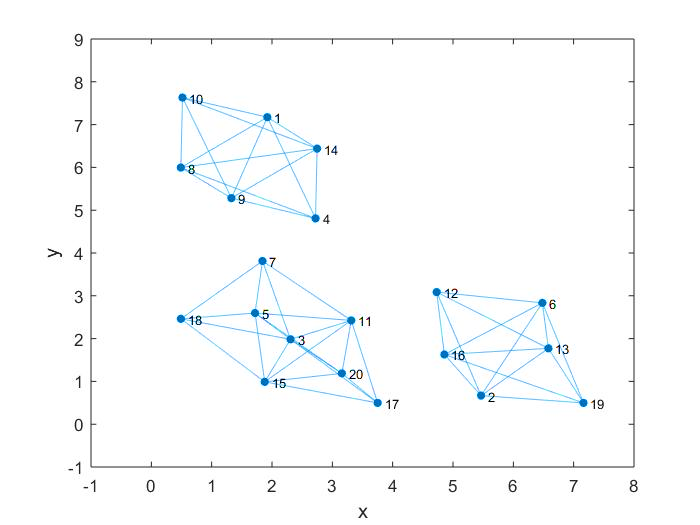
\includegraphics[width=0.5\linewidth]{graph.png}
	\caption{An example of the neighborhood graph representation among set-descriptor centroids.}
	\label{fig:graph}
\end{figure}

After each standard update (Eq.~\eqref{eq:update_mean}), every centroid is additionally smoothed toward its graph neighbors, proportionally to distance:
\begin{equation}
	\label{eq:cluster_centroid}
	\hat{\mu}_j = \frac{\sum_{l=1}^{N_j} w_l \mu_l}{\sum_{l=1}^{N_j} w_l}, \qquad w_l = \exp(-\beta d_{jl}),
\end{equation}
where $\hat{\mu}_j$ is the smoothed descriptor mean for set $j$, $N_j$ is its number of graph neighbors, $\mu_l$ is neighbor $l$'s mean, $d_{jl}$ is the feature-space distance between descriptors $j$ and $l$, and $\beta > 0$ is a dataset-specific damping constant preventing any single neighbor from dominating the update. This regularization limits the impact of outlier evidence on any one descriptor, controlling abrupt changes and yielding a more robust streaming realization of $\theta_j$.

\subsection{Latent-Filtered Rating Prediction and Top-\textit{N} Recommendation}
\label{subsec:rating_prediction}

Given a target user's membership degrees $u_{ij}$ — either previously computed (existing user) or freshly computed via Eq.~\eqref{eq:update_u} (new user) — the predicted rating for a candidate item is obtained by averaging the ratings assigned to that item by the user's neighbors within the sets to which they belong with non-negligible membership, directly instantiating the relevance-driven selection rule of Eq.~\eqref{eq:estimated_set}:
\begin{equation}
	\label{eq:avgrating}
	\hat{r} = \frac{1}{C \times M} \sum_{j=1}^{C} \sum_{l=1}^{M} r_{jl},
\end{equation}
where $C$ is the number of sets the target user belongs to with non-negligible membership and $M$ is the number of neighbors considered per set. After predicting scores for all candidate items, the top-$N$ items by predicted rating are recommended; following common practice, we use $N = 5$.

\begin{figure}[t]
	\centering
	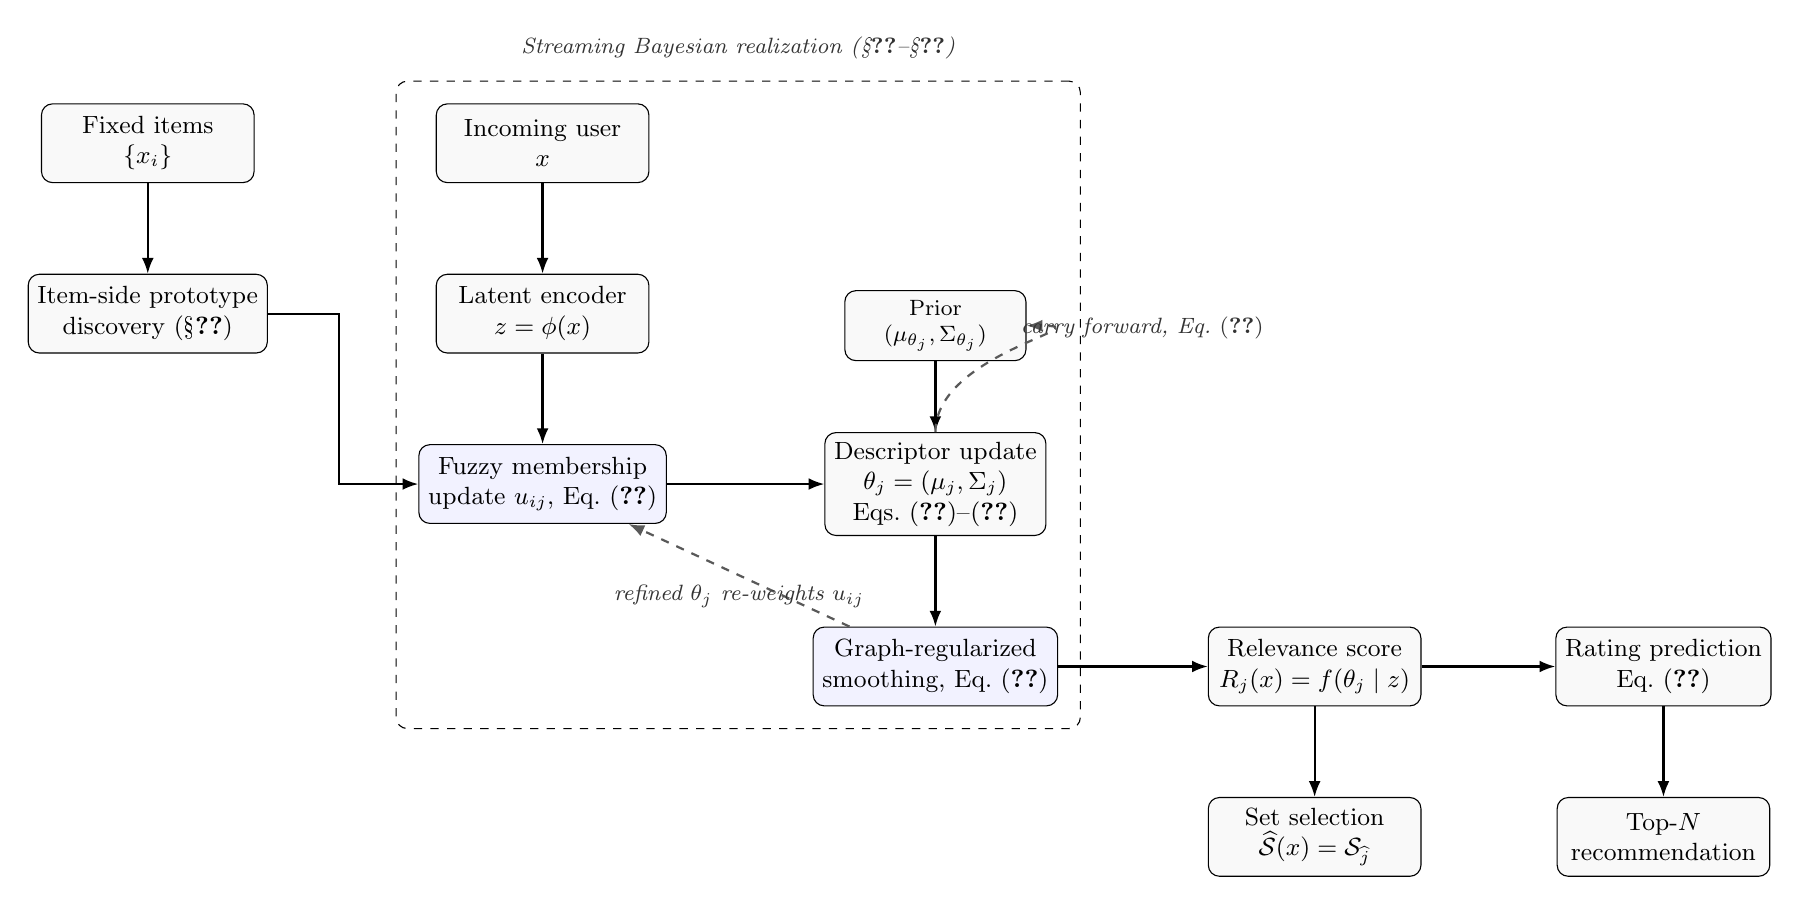
\begin{tikzpicture}[
		node distance=1.15cm and 1.5cm,
		box/.style={draw, rounded corners, align=center, minimum width=2.7cm, minimum height=1.0cm, font=\small, fill=gray!5},
		smallbox/.style={draw, rounded corners, align=center, minimum width=2.3cm, minimum height=0.85cm, font=\footnotesize, fill=gray!5},
		decision/.style={draw, rounded corners, align=center, minimum width=2.6cm, minimum height=1.0cm, font=\small, fill=blue!5},
		arrow/.style={-{Latex[length=2mm]}, thick},
		feedback/.style={-{Latex[length=2mm]}, thick, dashed, gray!70!black},
		dashedbox/.style={draw, dashed, rounded corners, inner sep=8pt},
		phase/.style={font=\footnotesize\itshape, gray!40!black}
		]
		\node[box] (items) {Fixed items\\ $\{x_i\}$};
		\node[box, below=of items] (fcm) {Item-side prototype\\ discovery (\S\ref{subsec:item_clustering})};
		
		\node[box, right=2.3cm of items] (user) {Incoming user\\ $x$};
		\node[box, below=of user] (enc) {Latent encoder\\ $z=\phi(x)$};
		
		\node[decision, below=of enc] (membership) {Fuzzy membership\\ update $u_{ij}$, Eq.~\eqref{eq:update_u}};
		
		\node[box, right=2.0cm of membership] (descriptor) {Descriptor update\\ $\theta_j=(\mu_j,\Sigma_j)$\\ Eqs.~\eqref{eq:update_mean}--\eqref{eq:update_cov}};
		
		\node[smallbox, above=0.9cm of descriptor] (prior) {Prior\\ $(\mu_{\theta_j},\Sigma_{\theta_j})$};
		
		\node[decision, below=of descriptor] (graph) {Graph-regularized\\ smoothing, Eq.~\eqref{eq:cluster_centroid}};
		
		\node[box, right=1.9cm of graph] (score) {Relevance score\\ $R_j(x)=f(\theta_j\mid z)$};
		
		\node[box, below=of score] (select) {Set selection\\ $\widehat{\mathcal S}(x)=\mathcal S_{\widehat j}$};
		
		\node[box, right=1.7cm of score] (rating) {Rating prediction\\ Eq.~\eqref{eq:avgrating}};
		
		\node[box, below=of rating] (topn) {Top-$N$\\ recommendation};
		
		\draw[arrow] (items) -- (fcm);
		\draw[arrow] (fcm.east) -| ++(0.9,0) |- (membership.west);
		
		\draw[arrow] (user) -- (enc);
		\draw[arrow] (enc) -- (membership);
		\draw[arrow] (membership) -- (descriptor);
		\draw[arrow] (descriptor) -- (graph);
		\draw[arrow] (graph) -- (score);
		\draw[arrow] (score) -- (select);
		\draw[arrow] (score) -- (rating);
		\draw[arrow] (rating) -- (topn);
		
		\draw[arrow] (prior) -- (descriptor);
		\draw[feedback] (descriptor.north) .. controls +(0,1.0) and +(1.0,0) .. (prior.east)
		node[midway, above right, phase] {carry forward, Eq.~\eqref{eq:update_prior}};
		\draw[feedback] (graph) -- (membership) node[midway, below, phase] {refined $\theta_j$ re-weights $u_{ij}$};
		
		\node[dashedbox, fit=(user)(enc)(membership)(descriptor)(prior)(graph)] (streambox) {};
		\node[phase, above=0.15cm of streambox] {Streaming Bayesian realization (\S\ref{subsec:user_clustering}--\S\ref{subsec:distributed_clustering})};
		
	\end{tikzpicture}
	\caption{Streaming latent-filtering recommendation pipeline. Item-side prototypes are discovered once, offline (left), while user-side set descriptors $\theta_j$ are realized online through an alternating Bayesian loop: incoming users update fuzzy memberships $u_{ij}$ and descriptors $\theta_j$, which are graph-regularized and fed back as priors for the next arrival (dashed feedback arrows). The resulting descriptors instantiate the general relevance score $R_j(x)$ of Eq.~\eqref{eq:collapsed_relevance}, used both for set selection and for rating-based top-$N$ recommendation.}
	\label{fig:recommender_flow}
\end{figure}

\subsection{Theoretical Analysis of the Streaming Estimator}
\label{subsec:theory}

\subsubsection{Convergence of the Streaming Estimator}

The objective $J_m$ (Eq.~\eqref{eq:obj_function}) is optimized by alternating between updating the membership matrix $u$ (Eq.~\eqref{eq:update_u}) and updating the set descriptors $\theta_j$ (Eqs.~\eqref{eq:update_mean}--\eqref{eq:update_cov}), holding the other block fixed at each step — a block-coordinate (alternating) minimization scheme in the same family as classical FCM. Convergence follows from the generalized convergence theorem of Zangwill together with the local-convergence result of \cite{hathaway1986local}: provided (i) each subproblem — minimizing $J_m$ over $u$ with $\theta$ fixed, and over $\theta$ with $u$ fixed — has a unique, continuous solution (guaranteed here, since Eq.~\eqref{eq:update_u} and Eqs.~\eqref{eq:update_mean}--\eqref{eq:update_cov} are closed-form and continuous in their inputs), and (ii) the iterates are initialized sufficiently close to a stationary point of $J_m$, the sequence $\{u^{(k)}, \theta^{(k)}\}$ converges to a local minimum of $J_m$ — by Proposition~\ref{prop:map_ml}, a local MAP/ML estimate of the set descriptors.

Condition (ii) motivates the initial (non-streaming) clustering pass in Section~\ref{subsec:item_clustering}: performing item-side clustering before entering the streaming loop places the iterates close to a minimum of $J_m$ from the outset, rather than relying on convergence from an arbitrary random start.

\subsubsection{Convergence Rate}

We next characterize how quickly a set descriptor's mean stabilizes under the streaming update. From Eq.~\eqref{eq:update_mean}, incorporating a new sample $z_{n+1}$ into set $j$ yields the recursion
\begin{equation}
	\label{eq:mu_recursion}
	\mu_{n+1} = S \, \mu_n + (1-S) \, z_{n+1} + M,
\end{equation}
where, from Eqs.~\eqref{eq:update_mean}--\eqref{eq:aux_S}, $S = \sum_{i=1}^{n} u_{ij}^m f_{ij} \big/ \sum_{i=1}^{n+1} u_{ij}^m f_{ij} \in [0,1)$ is the fraction of accumulated evidence mass contributed by previously seen samples, and $M$ collects the bounded prior-pull term.

Equation~\eqref{eq:mu_recursion} is a first-order linear recursion, i.e., a discrete-time contraction whenever $S \in [0,1)$. Unrolling it $k$ steps from an initial mean $\mu(0)$ gives the closed form
\begin{equation}
	\label{eq:mu_k}
	\mu(k) = S^{k}\mu(0) + \sum_{i=1}^{k} S^{\,k-i}(1-S)\,z(i) + \sum_{i=1}^{k} S^{\,k-i} M(i).
\end{equation}
Let $\mu^\star$ denote the fixed point of the recursion. Subtracting the fixed-point relation from Eq.~\eqref{eq:mu_recursion} gives
\begin{equation}
	\label{eq:error_recursion}
	\mu(k) - \mu^\star = S^k \big(\mu(0) - \mu^\star\big) + O\!\big((1-S)\big),
\end{equation}
so the deviation from the fixed point decays geometrically with rate $S$: $\|\mu(k) - \mu^\star\| = O(S^k)$. Because $S$ is the fraction of evidence mass attributable to \emph{previously accumulated} samples, $S$ is smaller — and hence convergence is faster — precisely when the streaming update weighs incoming evidence more heavily relative to accumulated history, the regime induced by the proposed Bayesian weighting in Eq.~\eqref{eq:aux_S}. This gives a direct, closed-form account of the faster empirical convergence of the proposed method relative to standard FCM (Fig.~\ref{fig:cn-rate}): both follow a recursion of the form of Eq.~\eqref{eq:mu_recursion}, but differ in the effective contraction rate $S$ induced by their respective weighting schemes.

\begin{figure}
	\centering
	\begin{subfigure}[b]{0.45\textwidth}
		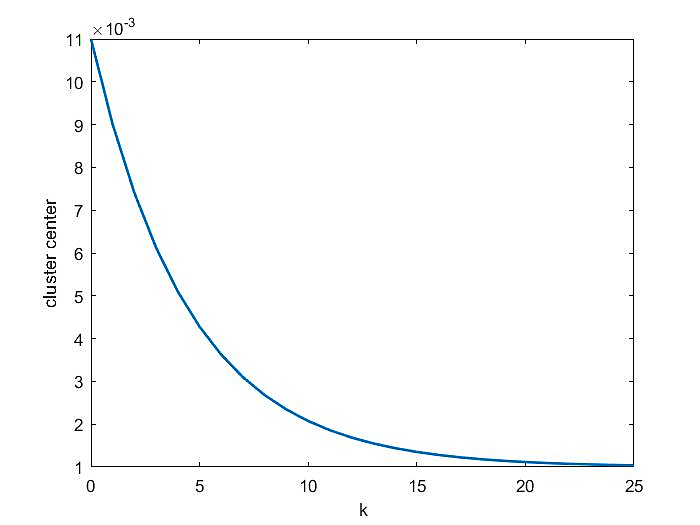
\includegraphics[width=\textwidth]{Cnrate_FCM.png}
		\caption{FCM}
	\end{subfigure}
	\begin{subfigure}[b]{0.45\textwidth}
		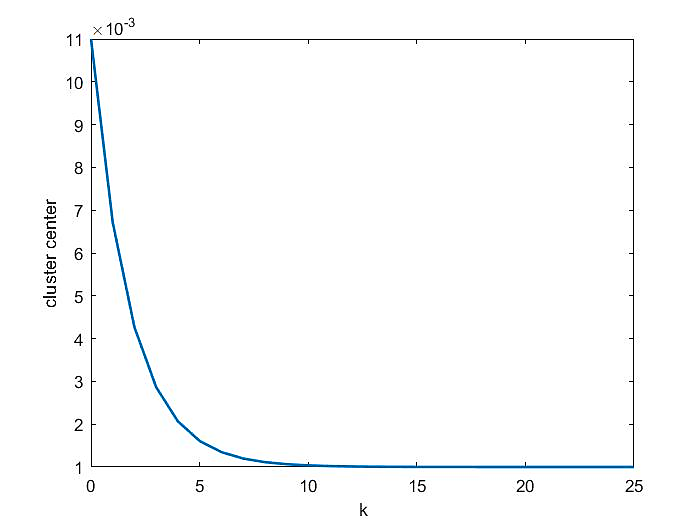
\includegraphics[width=\textwidth]{Cnrate_pmethod.png}
		\caption{Proposed method}
	\end{subfigure}
	\caption{Comparison of empirical convergence rates of the proposed clustering method and FCM. Both follow the geometric decay predicted by Eq.~\eqref{eq:error_recursion}; the proposed method attains a smaller effective contraction rate $S$, yielding faster convergence.}
	\label{fig:cn-rate}
\end{figure}






























% ************************************************************************




























\section{Experiments}
In this section, we investigate the accuracy and performance of the proposed method on various datasets. A comparative analysis with other methods as well as a discussion in parameter setting  is presented.

\subsection{Data sets}
The proposed recommender system was evaluated on the widely used MovieLens-100k, and MovieLens-1M and Yelp datasets, which are standard benchmarks in recommender system methods.
The MovieLens dataset includes user ratings and movie features collected from the MovieLens website, with movies categorized by genre. Preprocessing converted genres into binary indicators, where 1 denotes genre membership and 0 otherwise. The study utilizes MovieLens 100K, which includes 100,000 ratings from 1,000 users across 1,700 movies, and MovieLens 1M, containing 1 million ratings from 6,000 users for 4,000 movies, with additional user attributes such as age, gender, and occupation. These attributes are used for clustering in recommendation models.

The Yelp dataset features information on businesses across 11 cities in 4 countries, focusing on the restaurant category. It includes 4 million reviews from 1 million users for 58,000 restaurants, with detailed restaurant features (e.g., parking, child-friendliness, ambiance) and user attributes (e.g., age, gender, and average rating). Restaurant features were converted into numerical values (0 for absence, 1 for presence, and -1 for unspecified).

\subsection{Evaluation criteria}
Recommender systems are typically evaluated using two categories of criteria, prediction accuracy and decision support. Prediction accuracy metrics, such as Mean Absolute Error (MAE) and Root Mean Squared Error (RMSE), measure the numerical accuracy of predicted ratings. 

\begin{equation}
    \text{MAE} = \frac{1}{|S|} \sum_{i=1}^{|S|} |pred_i - r_i|
\end{equation}


\begin{equation}
    \text{RMSE} = \sqrt{\frac{1}{|S|} \sum_{i=1}^{|S|} (pred_i - r_i)^2}
\end{equation}

where, $pred_i$ and $r_i$ are the predicted and real scores for item $i$ respectively, and $|S|$ is number of test data.

In contrast, decision support metrics, including precision, recall, and F1 score, evaluate the system's effectiveness in providing relevant recommendations. Predicted scores for the items determined whether an item should be considered relevant and recommended to the target user or not. With a score range of 1 to 5, items rating $\leq 3$ are classified as irrelevant, while those rating $\geq 4$ are considered relevant. Therefore, precision, defined as the ratio of relevant suggested items to the total suggested items, ensures that recommendations are relevant and minimize unnecessary suggestions. Recall is the ratio of suggested relevant items to the total number of relevant items. F1 is a combination of precision and recall. These are defined as follows
\[
\text{Precision} = \frac{\#tp}{\#tp + \#fp}
\]

\[
\text{Recall} = \frac{\#tp}{\#tp + \#fn}
\]

\[
F1 = \frac{2 \times P \times R}{P + R}
\]
where, tp denotes the items suggested to the user by the recommendation system based on the predicted score, that are also relevant according to the actual score. Similarly, fp , fn and tn represent the suggested irrelevant items, not suggested relevant items and not suggested irrelevant items, respectively.


\subsection{Evaluation of the Proposed Recommender System}
To assess the accuracy of the proposed recommender system and compare the effectiveness of the proposed approach, its performance was benchmarked against existing clustering-based recommendation methods, including \cite{liji2018improved, kant2017leaderrank, mohammadpour2019efficient, wasid2018clustering}. Table \ref{tab:comparison_results} presents the comparison results for different methods using the evaluation criteria on the MovieLens-100K, MovieLens-1M, and Yelp datasets.

\begin{table}[htbp]
\centering
\caption{Comparison of the Proposed Method with others}
\label{tab:comparison_results}
\renewcommand{\arraystretch}{1.3}
\setlength{\tabcolsep}{3pt}
\begin{tabular}{clccccc}
\hline
\textbf{Data Sets} & \textbf{Method} & \textbf{MAE} & \textbf{RMSE} & \textbf{Precision} & \textbf{Recall} & \textbf{F1} \\
\hline
\multirow{5}{*}{ML\_100K} & Chen\cite{liji2018improved} & 0.74 & 0.95 & 0.88 & 0.50 & 0.642 \\
& Kant\cite{kant2017leaderrank} & 0.75 & 0.95 & 0.56 & 0.87 & 0.681 \\
& Enayatifar \cite{mohammadpour2019efficient} & 0.78 & 0.96 & - & - & - \\
& Wasid \cite{wasid2018clustering} & 0.91 & 1.12 & 0.54 & 0.75 & 0.627 \\
& \textbf{Proposed Method} & \textbf{0.71} & \textbf{0.91} & 0.56 & 0.89 & \textbf{0.687} \\
\hline
\multirow{5}{*}{ML\_1M} & Chen & 0.72 & 0.94 & 85.3 & 0.49 & 0.622 \\
& Kant & 0.72 & 0.925 & 0.53 & 0.86 & 0.653 \\
& Enayatifar & 0.85 & 1.35 & - & - & - \\
& Wasid & 0.95 & 1.24 & 0.56 & 0.71 & 0.626 \\
& \textbf{Proposed Method} & \textbf{0.705} & \textbf{0.925} & 0.62 & 0.85 & \textbf{0.71} \\
\hline
\multirow{3}{*}{Yelp} & Kant & 0.965 & 1.25 & 0.57 & 0.78 & 0.65 \\
&  \textbf{Proposed Method} & \textbf{0.943} & \textbf{1.21} & 0.61 & 0.81 & \textbf{0.69} \\
\hline
\end{tabular}
\end{table}

In all the mentioned methods, a clustering model has been used to find users or similar items and finally predict the score for the users. Also, in all these studies, the number of data has been assumed to be constant. According to the comparison, it is observed that although the proposed method considers the data as online and streaming, it has better performance than other methods.

Furthermore, to evaluate the feasibility of the proposed method for real-time applications, we analyzed the computation time required for rating predictions. Table \ref{tab:computation_time} presents the comparison between the proposed method and the approach \cite{kant2017leaderrank} in terms of maximum computational time required per prediction in three datasets. It is evident that the proposed method performs efficiently compared to existing approaches. Its speed makes it suitable for deployment in real-world systems with streaming data.

\begin{table}[h]
\centering
\caption{Computational Time Comparison (in milliseconds)}
\label{tab:computation_time}
\renewcommand{\arraystretch}{1.3}
% \setlength{\tabcolsep}{2pt}
\begin{tabular}{lccc}
    \hline
    \textbf{Method} & \textbf{Yelp} & \textbf{MovieLens-100K} & \textbf{MovieLens-1M} \\
    \hline
    Kant et al. [43] & 48 ms & 18 ms & 25 ms \\
    \textbf{Proposed Method} & \textbf{50 ms} & \textbf{22 ms} & \textbf{28 ms} \\
    \hline
\end{tabular}
\end{table}

\subsection{comparision with standard FCM}

For comparing the final performance and convergence speed of the proposed clustering method versus the standard FCM, the FCM objective function's value is computed separately for both methods per iteration. This allows for a proper comparison, even though each method updates parameters differently and has its own unique objective function. The convergence speed comparison for every dataset can be seen in Figure \ref{fig:combined}.

\begin{figure}[H]
\centering
% Subfigure 1
\begin{subfigure}[b]{0.3\textwidth}
    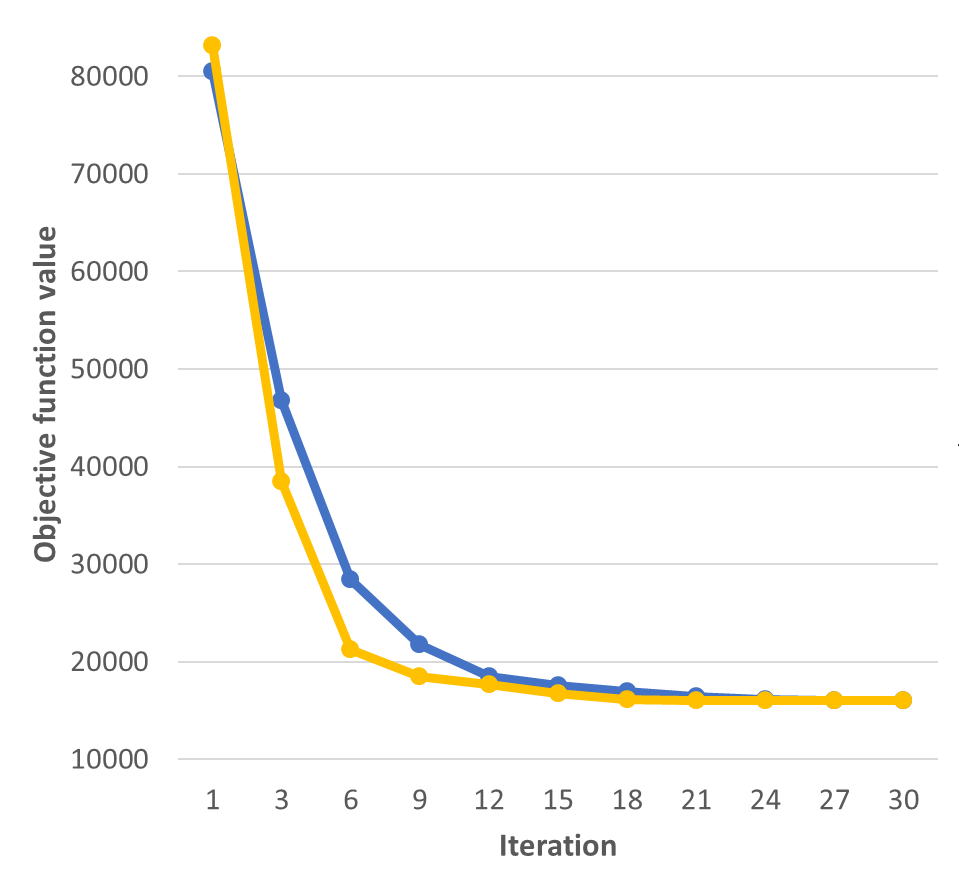
\includegraphics[width=\textwidth]{fcm1final.png}
    \caption{M\_100K}
    % \label{fig:sub1}
\end{subfigure}
\hfill
% Subfigure 2
\begin{subfigure}[b]{0.3\textwidth}
    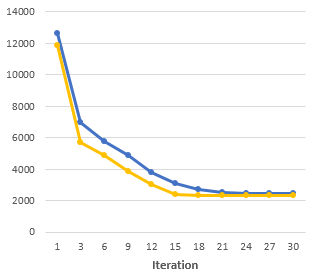
\includegraphics[width=\textwidth]{fcm2final.PNG}
    \caption{ML\_1M}
    % \label{fig:sub2}
\end{subfigure}
\hfill
% Subfigure 3
\begin{subfigure}[b]{0.3\textwidth}
    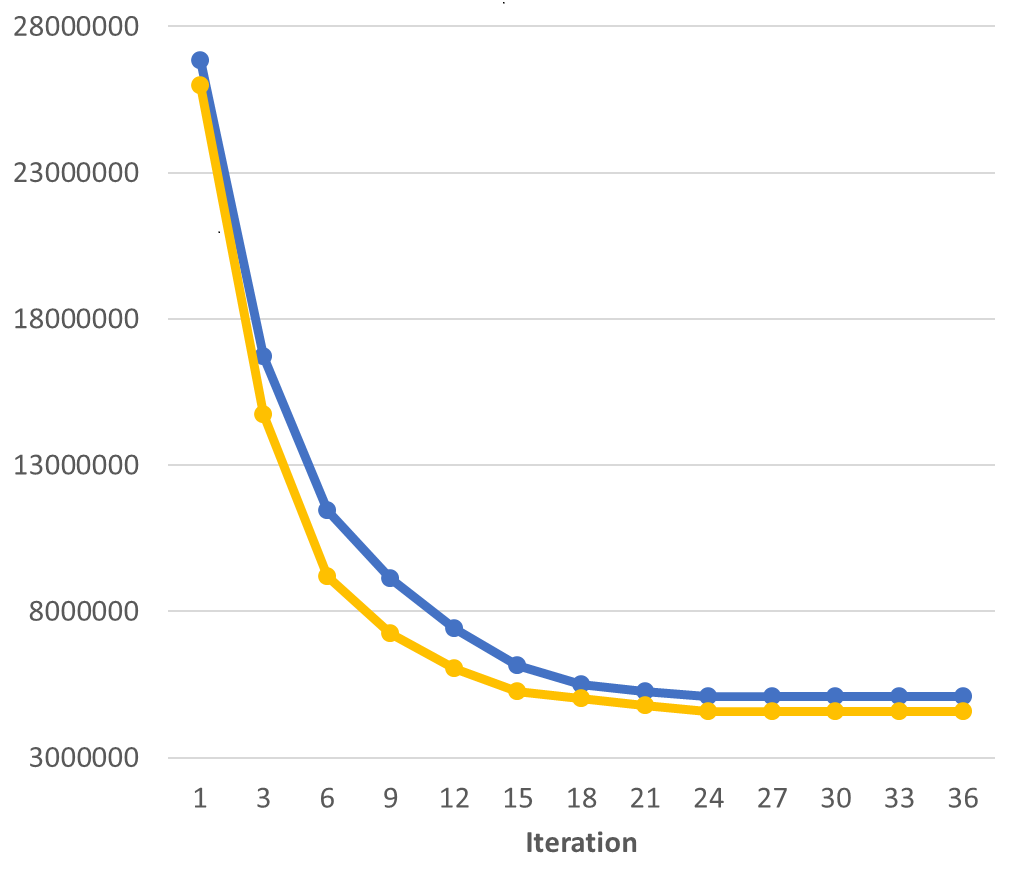
\includegraphics[width=\textwidth]{fcm3final.png}
    \caption{Yelp}
    % \label{fig:sub3}
\end{subfigure}

\caption{Comparison of the convergence rate and speed of the proposed method and the FCM method on the different datasets. Blue and yellow line denotes the FCM and proposed method respectively}
\label{fig:combined}
\end{figure}


Table \ref{tab:cmpFCM} compares both methods based on the minimum FCM objective function value attained and the minimum iterations required. The comparison demonstrates that the proposed method outperforms FCM by converging faster and lowering the objective function value more substantially.

\begin{table}[htbp]
\centering
\caption{Comparison of the proposed method with FCM}
\label{tab:cmpFCM}
\renewcommand{\arraystretch}{1.3}
\setlength{\tabcolsep}{8pt}
\begin{tabular}{lcccc}
\hline
% \rowcolor[gray]{0.9}
\textbf{Data set} & \multicolumn{2}{c}{\textbf{FCM}} & \multicolumn{2}{c}{\textbf{Proposed method}} \\
\cline{2-5}
& \textbf{value} & \textbf{iterations} & \textbf{value} & \textbf{iterations} \\
\hline
ML-100K & 2709 & 18 & 2402 & 15 \\
ML-1M   & 16099 & 22 & 16093 & 19 \\
% \rowcolor[gray]{0.9}
Yelp    & 5078242 & 26 & 4587557 & 23 \\
\hline
\end{tabular}
\end{table}



\subsection{Parameter Discussion}
To assess the effect of different parameter settings on performance, we conducted experiments to analyze the impact of number of cluster and the percentage of data used in initial clustering. 
Initially, 80\% of the data is randomly selected as training data, while the remaining 20\% is used for testing.
Then, a portion of the training data is allocated for initial clustering and parameter setting. Consequently, both the number of user clusters and the proportion of data used for this initial phase influence the quality of the clustering results.
Table \ref{tab:parameter_discussion} presents the prediction accuracy of the proposed recommender system across different numbers of user clusters and considering two data usage scenarios: 30\% and 40\% of the training data.

The results indicate that using 40\% of the data for initial clustering leads to more effective user clustering, which enhances the overall prediction accuracy.

\begin{table}[htbp]
\centering
\caption{Accuracy of the proposed method across different parameter settings}
\label{tab:parameter_discussion}
\renewcommand{\arraystretch}{1.3}
\setlength{\tabcolsep}{3pt}
\begin{tabular}{cccccccccc}
\hline
\multirow{2}{*}{\textbf{Datasets}} & \multirow{2}{*}{\begin{tabular}[c]{@{}c@{}} initial \\ data\end{tabular}} & \multicolumn{2}{c}{\textbf{60}} & \multicolumn{2}{c}{\textbf{80}} & \multicolumn{2}{c}{\textbf{100}} & \multicolumn{2}{c}{\textbf{110}} \\
\cline{3-10}
 &  & MAE & RMSE & MAE & RMSE & MAE & RMSE & MAE & RMSE \\
\hline
\multirow{2}{*}{ML\_100K} & 30\% & 0.73 & 0.925 & 0.72 & 0.92 & 0.76 & 0.955 & - & - \\
 & 40\% & 0.73 & 0.917 & \textbf{0.71} & \textbf{0.91} & 0.74 & 0.96 & - & - \\
\hline
\multirow{2}{*}{ML\_1M} & 30\% & 0.78 & 1.0 & 0.763 & 0.979 & 0.72 & 0.95 & 0.725 & 0.935 \\
 & 40\% & 0.77 & 0.98 & 0.752 & 0.976 & \textbf{0.705} & \textbf{0.925} & 0.718 & 0.93 \\
\hline
\multirow{2}{*}{Yelp} & 30\% & 0.993 & 1.45 & 0.975 & 1.43 & 0.965 & 1.31 & 0.955 & 1.32 \\
 & 40\% & 0.99 & 1.47 & 0.965 & 1.40 & 0.945 & 1.25 &\textbf{0.943} &\textbf{1.21} \\
\hline
\end{tabular}
\end{table}


In addition, based on these comparisons, the optimal number of clusters for users in each data set is determined. According to the results obtained, the optimal number of clusters for the MovieLens\_100k data set is 80 clusters, for the MovieLens\_1M data set is 100 clusters, and for the yelp data set is 110 clusters.

Also, according to the experiments conducted, the optimal number of clusters for items in the MovieLens dataset, due to the limited number of genres, was 20 clusters and in the Yelp dataset, 80 clusters.

These findings confirm that the proposed Bayesian clustering model outperforms traditional clustering approaches while maintaining low computational overhead, making it well-suited for real-time recommender systems.

\section{Conclusion}
In this study, a method based on the Bayesian clustering model is used. Initially, to reduce the feature for user clustering, the items are clustered using FCM. Then, As considering the users are not constant and added to the system dynamically, a Bayesian clustering method is used for user clustering. In this approach, learning is conducted in a distributed manner, where cluster centroids interact and influence each another based on their relative distances. This minimizes the impact of outliers on the cluster centroids. Finally, after clustering, the scores of neighboring users are used to predict a user's score on an item that they have not seen yet, and the items with the highest scores are suggested to each user. The evaluation results on streaming data events demonstrate that the proposed method outperforms existing approaches in enhancing recommender system performance, achieving more precise user score predictions. In proposed method, items are considered constant, which is a limitation in real-world application. Future research could address this by considering dynamic item. Furthermore, integrating a score prediction methods that utilize both user-user and item-item similarities could enhance recommendation accuracy.

% \bibliographystyle{plain} % Specify the bibliography style
% \bibliography{RecommendationBib.bib}
\printbibliography

\end{document}

% F. Maxwell Harper and Joseph A. Konstan. The movielens datasets: Historyand context. ACM Trans. Interact. Intell.
Syst., 5(4):19:1–19:19, 2016.